
\paragraph{Mixture Modeling}\label{para:MixtureModeling}

To assess the bias in responses for each cue, we computed the distribution of responses on trials where the monkey made an incorrect choice.
For each completed trial, we calculated the error as the angular difference between the correct option and the chosen option.  
For each cue, we computed the number of times the monkey selected each incorrect choice, normalized by the number of times each choice color was available as a choice option for all completed trials of the given cue (though this was approximately uniformly distributed).
We then fit a Gaussian with a variable floor (\autoref{eq:GaussianEquation}) to the error distribution for each cue, using the MATLAB \lstinline{fit} function with the equation defined as \lstinline{a*exp(-(((x-b)^2)/(2*c^2)))+d}. 

% demo annotated-equation code from here: https://mirrors.concertpass.com/tex-archive/macros/latex/contrib/annotate-equations/annotate-equations.pdf

%\newpage %Sometimes the annotations don't show up, the hacky solution is to force them onto a new page

\vspace{2em} 
\begin{equation} \label{eq:GaussianEquation}
    \eqnmarkbox[purple]{p1}{a}
    \cdot
    \exp
    \frac{-(x-
    \eqnmarkbox[violet]{mu}{\mu}
    )^2}{2 
    \eqnmarkbox[blue]{sigma}{\sigma}^2}
    +
    \eqnmarkbox[gray]{d}{d}        
\end{equation}

\annotate[yshift=1em]{above,left}{p1}{height of the curve's peak}
\annotate[yshift=1em]{above}{mu}{position of the center of the peak}
\annotate[yshift=-0.75em]{below,left}{sigma}{standard deviation}
\annotate[yshift=-1em]{below}{d}{floor}
\vspace{2em} 

This fit was weighted by the number of times each choice color was an option for the given cue across all completed trials (though as before, this was approximately uniformly distributed). 
Bias was taken as the difference between the cue and the peak of the corresponding Gaussian, for each cue color ($b$ in \autoref{eq:GaussianEquation}). 
%These values were then smoothed (with a circular moving average filter of 5 cues) since our primary interest was in the broader structure of the bias distribution, and this is shown as the black lines in \autoref{fig:BiasCurves}.
These values, for each stimulus, are plotted as the black lines in \autoref{fig:BiasCurvesCombined}.
Where this line falls closer to the center of the figure than the 0$^{\circ}$ line, there is negative bias (which in this representation is counter-clockwise), and vice versa for values above the 0$^{\circ}$ line.
%Attractor points (thought to indicate color category centers) occur where the bias curve crosses the zero line from positive to negative (going counter-clockwise).
%At these points, there is zero bias, and hues on either side provoke choices that are biased inwards towards this point.
%Correspondingly, repeller points occur where the bias curve crosses the zero line from \emph{negative to positive} (again, going counter-clockwise).
%At these points there is also zero bias, but hues either side of this point are biased \emph{away} from this point.
Confidence intervals were extracted from 

%\subparagraph{Confidence intervals}
%To find the 95\% confidence intervals for the locations of the category centers, we performed 1000 bootstraps on all completed trials. For each bootstrapped sample, we found the bias values for each cue color, smoothed the bias curve, and found the category center locations for each bootstrapped dataset. To find the category center locations for the full data set and their confidence interval, we found the category boundaries and segmented all bootstrapped category centers that fell between two consecutive category boundaries. For each of these segments, we found the circular mean and circular standard deviation of all category crossings that fell within these boundaries. 
%\begin{figure}
%\includesvg[inkscapelatex=false, width=\textwidth]{../../Figures/F2_DataAnalysis_v2.svg}
%\caption{\textbf{Task performance.}
%Performance as a function of trial difficulty, quantified as the closeness of the chromatically closest incorrect choice.
%\emph{A.} For one animal, with five example choice sets below for trials where the cue was cue \#28 (correct choice highlighted by dashed line here, not visible to animal).
%\emph{B.} For all animals.
%} 
%\label{fig:TaskPerformance}
%\end{figure}

\paragraph{Target Confusability Competition (TCC)}\label{para:TCC}
One disadvantage of the mixture model for our analysis is that we can only use it to analyze the subset of trials where the animal made an incorrect response\footnote{
This is for messy and annoying reasons. 
Firstly, since in our paradigm the choices consist of ``the correct choice'' plus three ``distractors'' (see \nameref{para:4AFC}), the correct choices are greatly over-represented. 
Imagine: by guessing at random, the correct choice would be picked far more frequently than any of the other stimuli, since it is presented on \emph{every trial}, whereas the other stimuli are only presented as distractors with a probability of $\frac{1}{63} + \frac{1}{62} + \frac{1}{62}$. 
This could be normalized out, as we do for the other values, but then a more insidious issue becomes apparent: 
For ``high-error'' choices, the odds of there being a similar choice to that one is less than the odds of there being a similar choice to the ``0-error'' choice, and thus the probability of selecting the correct answer, when normalised, is lower than one would expect. 
%Or to flip the logic: there are slightly higher odds of there being a close distractor to the 0-error stimulus than there is to a high-error stimulus.
You can think of it as: for the high-error choice, there are \emph{2 chances} to pick another choice option that is close to the high-error choice (since one choice is going to be the distant-by-definition 0-error choice), whereas for the 0-error choice there are \emph{3 chances}.
%2 comes from: 1 already used to be the 0-error choice, which by definition is not close to the high-error choice. And 1 is the high error choice itself, so you have 2 left to place.
An additional note for clarity: this is an issue for us because of the sampling required for the AFC paradigm, and is not an issue of concern for those who use a response mechanism where all possible responses are simultaneously presented.
}.
In order to use the full dataset (both incorrect and correct trials), we developed a generative model, based on the \emph{Target Confusability Competition (TCC)} model of \cite{schurgin_psychophysical_2020}.
The key elements of the TCC model are a similarity function, which determines the similarity between stimulus $s_i$ and stimulus $s_j$ and a value of $d'$, which can be thought of as describing the amount of noise acting on the system. 
Taken together, these two elements can be used to predict the probability that a choice of colour $s_j$ will be picked, from the set of $[s_{j1} ... s_{jn}]$, on a trial where the cue is $s_i$.
Our implementation of the model differs in some key ways to that described in \cite{schurgin_psychophysical_2020}:
\begin{enumerate}
\item We do not assume that the underlying function is the same for each stimulus. 
\cite{schurgin_psychophysical_2020} collapse across stimuli for the majority of their analyses (though, see their Figures 1D and Extended Data Figure 5). 
Since we are most interested in the differences between the functions for the different stimuli, it does not make sense for us to collapse our data. 
We therefore deal with a ``similarity matrix'', whereas \cite{schurgin_psychophysical_2020} could refer to their collapsed version as a ``similarity function''.
\item We make no assumptions about the underlying function that determines similarity. \cite{schurgin_psychophysical_2020} use an exponential function with additional perceptual noise (see their Figure 1F), based on observations gained from collecting data on various simultaneous judgment tasks. We choose not to do this, because we expect that if biases are present, this would modify the shape of the function differently for each stimulus. We refer to fits made this way as ``free similarity matrix'' fits, since each elements of the matrix is ``free'' to float as it wishes, independently of those elements around it.
\item We fit our model on a single dataset, whereas \cite{schurgin_psychophysical_2020} derive their similarity functions and values for $d'$ from independent datasets. % why do they do this?
\item In fitting a ``free similarity matrix'' noise in the system can either be represented by the value of $d'$ or in modifying the ``contrast'' of the similarity matrix (the relationship between the highest values and the lowest values in the matrix), since we apply no constraints on the floor or peak of the function. 
We therefore assume a value of $d' = 1$ for free similarity matrix fits. %and only actively fit $d'% in (these other models)...
\item Since we use an AFC method, as opposed to a pseudo-continuous response space, we are able to take advantage of an alternative computational method for computing the probabilities of a particular choice being made.
We use the correction factors of \cite{mcgraw_common_1992} (their Table 3) to estimate the probability $P(X_1>max(X_2,X_3,X_4))$, where $X_{1:4}$ are samples from independent normal variables, with means representing the pairwise similarity values between $s_i$ and $s_j$, and variances determined by $d'$.
This decreases the runtime of our model by several orders of magnitude compared to the method used by \cite{schurgin_psychophysical_2020} (See the function \lstinline{modelPDF} in \lstinline{TCC_Code_InManuscriptOrder\Model\TCCUncorrelated.m} from \url{https://osf.io/j2h65/} for comparison).
\end{enumerate}

Using this model, we used parameter estimation techniques to construct a similarity matrix where each cell represented the similarity between stimulus $s_i$ and stimulus $s_j$. 
Such a similarity matrix is shown in \autoref{fig:SimilarityMatrixPollux} for a single animal (Monkey P).
This model, and this visualization method, allows us to assess not only the mean of the bias in the responses, but the shape of the response-bias-curve, which gives us an insight into the source of the bias.

\paragraph{Distinguishing between cognitive biases and biases arising from non-uniformity of stimulus space}

For these experiments, we used a nominally perceptually-uniform colorspace: CIELUV. 
This space has been derived psychophysically, with the goal of minimizing differences in perceptual non-uniformity across the space, for color differences of small magnitudes (the apparent color difference between two points in one part of the space should be equal to the apparent color difference between two points in another part of the space when that the cartesian distance between the two points in each case be the same).

However, non-uniformities within the space are known to exist (ref?), and uniformity for small color differences does not necessarily assure uniformity for larger color differences (ref? Teunissen?). % no color space is perfect etc
Likewise, uniformity for the conditions under which the psychometric measurements from which the space was determined (considering: spatial, temporal, spectral etc.) does not necessarily assure uniformity across all possible viewing conditions (ref).

With this in mind, it is reasonable to consider what the effect of residual non-uniformity might be on the results of our experiment. 
As discussed by \cite{panichello_error-correcting_2019} (their Figure S5) non-uniformities in colorspace could also potentially lead to systematic biases on tasks such as ours. % However, I think the they reach the opposite conclusion as we do...
The logic goes as follows: our points are uniformly distributed in our chosen space (\autoref{fig:StimuliAndParadigm}A), but if this space is actually non-uniform compared to the colorspace implicitly being used by an observer, then these same points will be \emph{non}-uniformly distributed in a hypothetical `perfect colorspace'. 
It follows that for each cue color, surrounding distractor points might actually be closer or further away than anticipated. 
If the nearest neighbors on one side of the cue are actually chromatically closer than the neighbors on the other side, one would expect these to be chosen at a higher frequency than the others, creating a systematic bias.
\cite{panichello_error-correcting_2019} lack a robust framework within which to test these ideas, and conclude that there would be no effect on their conclusions. We reach a contrary conclusion.

%Unfortunately, these biases act in a similar fashion and are difficult to separate from one another. One potential way to distinguish one type of bias from another is to consider the theoretical relationship between bias and variance: if biases arise due to non-uniformities in colorspace, we would expect the attractor points to also have the \emph{highest} variance in responses. This is because in the hypothetical `perfect space' these points are actually tightly clustered, and so in the presence of noise we can assume that they will be frequently picked over one another. Conversely, at attractor points in spaces where the bias results from categoricality, theory would predict that we would see the \emph{lowest} levels of variance - if these points are conceptualized as `magnets' or `valleys' then we would expect cumulative noise to preferentially return to the attractor point, reducing the variance in responses.

It is difficult to distinguish biases from different sources using the Mixture Modeling approach... %why?
% is it because TCC seperates out d' and simMatrix, whereas mixmod implicitly combines the two (by using a matrix that is directly "probability of choice"?)

This task becomes tractable in the TCC framework. (why?)
A reasonable definition of cognitive bias might be: an agent is more likely to pick choice $s_2$ as a match to cue $s_1$ than they are to select choice $s_1$ as a match to cue $s_1$, and that this behavior would not be reciprocal (they would not be more likely to pick choice $s_1$ as a match to cue $s_2$ than they are to select choice $s_2$ as a match to cue $s_2$).
By this definition, this type of bias would appear as spread or displacement away from the negative diagonal in the similarity matrix, that \emph{was not} symmetric across the negative diagonal (symmetry across the diagonal would represent reciprocity).
There are numerous ways that cognitive bias can be envisaged/implemented.
A cartoon example is shown in \autoref{fig:JustBias}.

Spread away from the negative diagonal which is mirrored across the diagonal represents non-uniformity of the stimulus space.
In areas where the behavioral space is oversampled, one would see spread away from the negative diagonal (adjacent colors are more similar than the average).
In areas that are undersampled, one would see a pinch into the negative diagonal (adjacent colors are less similar than the average).
A cartoon example is shown in \autoref{fig:JustColSpace}.

\begin{figure}
    \centering
    \begin{subfigure}[b]{0.49\textwidth}
         \centering
         \caption{}
         %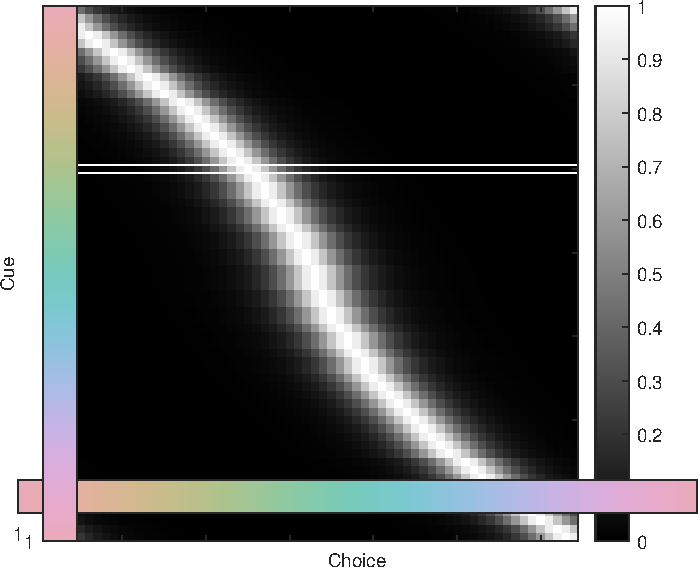
\includegraphics[width=\textwidth]{../../Figures/working/justBias.pdf}
         \includesvg[pretex=\tiny, width=\textwidth]{../../Figures/working/justBias.svg}
         \label{fig:JustBias}
    \end{subfigure}
    \hfill
    \begin{subfigure}[b]{0.49\textwidth}
         \centering
         \caption{}
         %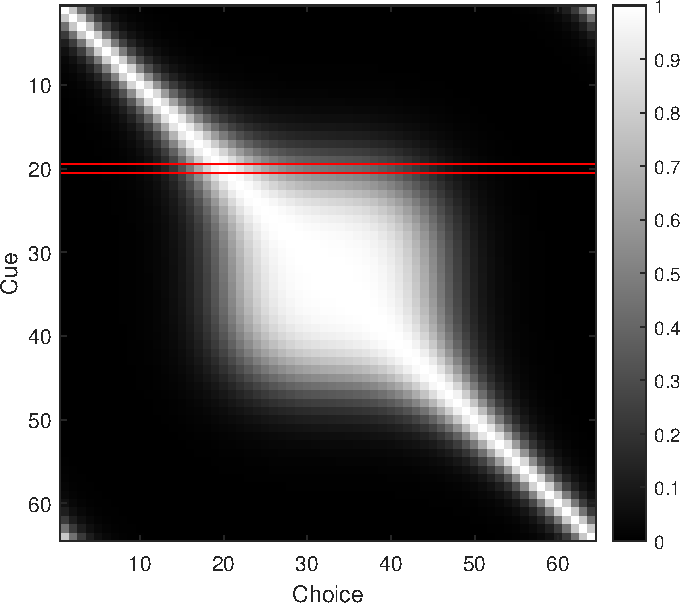
\includegraphics[width=\textwidth]{../../Figures/working/justColSpace.pdf}    
         \includesvg[pretex=\tiny, width=\textwidth]{../../Figures/working/justColSpace.svg}
         \label{fig:JustColSpace}
    \end{subfigure}

    \begin{subfigure}[b]{0.49\textwidth}
         \centering
         \caption{}
         %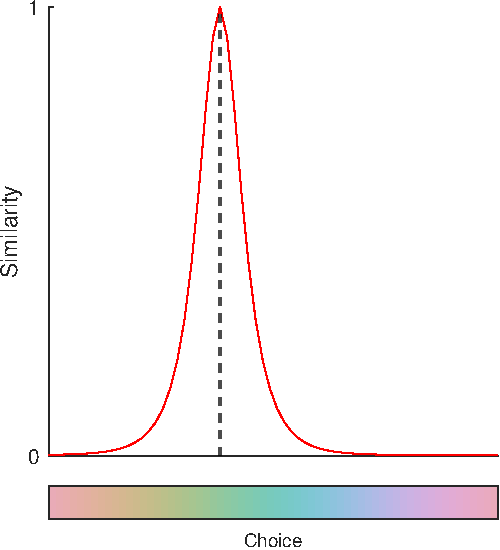
\includegraphics[width=\textwidth]{../../Figures/working/justBias_subset.pdf}
         \includesvg[pretex=\tiny, width=\textwidth]{../../Figures/working/justBias_subset.svg}
         \label{fig:JustBias_subset}
    \end{subfigure}
    \hfill
    \begin{subfigure}[b]{0.49\textwidth}
         \centering
         \caption{}
         %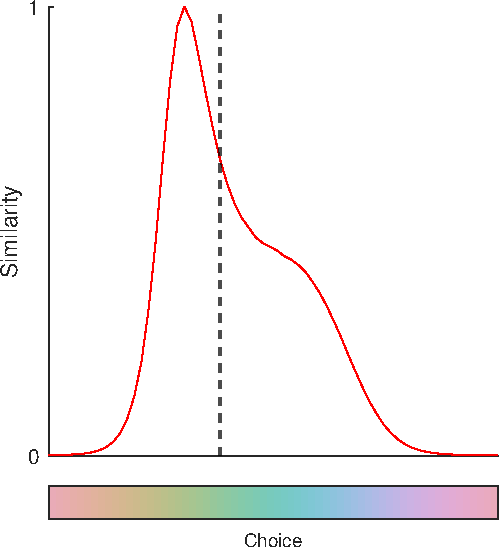
\includegraphics[width=\textwidth]{../../Figures/working/justColSpace_subset.pdf}
         \includesvg[pretex=\tiny, width=\textwidth]{../../Figures/working/justColSpace_subset.svg}
         \label{fig:JustColSpace_subset}
    \end{subfigure}
        \caption{\textbf{Distinguishing between different sources of bias using TCC models: cognitive bias vs. non-uniformity of stimulus space.} Similarity matrices representing different theoretically driven mechanisms can result in the same average bias value. A mixture model cannot distinguish between these different sources, whereas a TCC model readily can. \ref{fig:JustBias}: an example of how cognitive bias might appear - each row of the matrix is shifted leftwards or rightwards. \ref{fig:JustColSpace}: an example of how non-uniformity in stimulus space might appear - the similarity between each cue and its neighbors is increased or decreased, resulting in an expansion of the higher similarity region of the matrix symmetrically around the negative diagonal for colors which are more similar to their neighbors than average, and a contraction for colors that are less similar to their neighbors than average. \ref{fig:JustBias_subset}: The values representing the similarity function for cue 20 (the row highlighted in red in \ref{fig:JustBias}), with the circular median shown as a vertical dashed line. \ref{fig:JustColSpace_subset}: As in \ref{fig:JustBias_subset} but for \ref{fig:JustColSpace}. Note how the circular median of \emph{both} functions is 25}
        \label{fig:distinguishing}
\end{figure}

In this example, it is possible to see how responses could be biased even in the absence of cognitive bias - consider cue 20, for example. 
The similarity of cue 20 to all the possible choices is represented by the row of elements at location 20. Tracking left to right from the y-axis, see how there is only a small area of similarity to the left of the negative diagonal and a larger area of similarity to the right of the diagonal. 
Although the most similar choice is still 20, there is a longer tail of the similarity distribution to the right than to the left, and thus responses will be shifted to higher values on average. %illustrate? - by lines on graph, or by pulling out the individual? 

% this also affects standard deviation, which can be assessed in the mixture model...

To estimate how much of the bias could be attributed to non-uniformity of colorspace, we fit an alternative version of the TCC model. 
In this version, we use a single similarity function, defined by \autoref{eq:SimilarityFunction} (which is controlled by two parameters: $\lambda$ and $\sigma$, which together control the slope of the function and the extent of the flat-top of the function at zero)\footnote{These two parameters can be though of theoretically as the \emph{similarity function} (how similar is $x$ to $y$), and the \emph{perceptual function} (at what point do stimuli become indistinguishable from one-another). Unfortunately, in this parameterization of the function, the parameters are highly correlated, which makes recovery of these values via model fitting rather difficult. An alternative parameterization where the parameters were maximally uncorrelated would be preferable.} and instead allow the stimuli chromaticities to float.
This is akin to asking: what set of relationships between the stimuli in stimulus space can best explain the data we observe?
% do we fit the similarity function, or choose reasonable estimated values?

\renewcommand{\eqnhighlightheight}{\vphantom{\hat{H}}\mathstrut} %make the highlighted a standard height


\vspace{2em} 
\begin{equation} \label{eq:SimilarityFunction}
    \eqnmarkbox[purple]{explambda}{\exp(x\cdot\lambda)}
    \eqnmarkbox[cyan]{convolution}{\circledast}
    \eqnmarkbox[blue]{sigma}{\mathcal{N}(0,\sigma^2)}
\end{equation}

\annotate[yshift=1em]{above,left}{explambda}{scaled exponential}
\annotate{below,left}{convolution}{convolution}
\annotate[yshift=1em]{above}{sigma}{normal distribution with mean of 0 and standard deviation of $\sigma$}


% It would be possible to allow the stimuli to float in any number of dimensions, which might be useful for detecting luminance intrusion, or other unintended/unanticipated dimensions

% The rotation/offset in this space is arbitrary. It is all about relationships.

\vspace{2em} 

\paragraph{Reconstruction of colorspace}

...

%\begin{figure}
%\includesvg[inkscapelatex=false, width=\textwidth]{../../Figures/working/Poster_components/BiasCalculation copy.svg}
%\caption{Analysis and Hypotheses.} 
%\label{fig:BiasCalculation}
%\end{figure}


% Amazon Mechanical Turk Data

% Conversion between CIELAB and CIELUV

%\paragraph{Discrete vs. Continuous Response Space}
% MechTurk data vs. Bae/Panichello Humans
% Our monkeys vs. Panichello monkeys